\documentclass{article}
\usepackage{style}
\usepackage{MyNotations}
\begin{document}
\section{Modelling dislocations : An overview}
\subsection{Introduction to dislocations}
Crystals are a class of solid materials characterized by an ordered structure. Atoms occupy well defined sites in a pattern that repeats itself known as the \emph{crystal structure}. In fact, the arrangement of atoms in a crystal can be described by a three-dimensional network of parallel lines, forming equal-sized parallelepipeds. The points where these lines intersect define a \emph{Bravais} lattice, where each point has identical surroundings. A unit cell is the basic parallelepiped, and a crystal is formed by stacking identical unit cells in perfect alignment. By placing a group of atoms (motif) at each lattice point, the regular structure of a perfect crystal is created. This description only holds true for perfect crystal; however, in reality, crystals never are, and they suffer from several defects such as point-like, line, surface and even volume or bulk defects which renders them imperfect.\\ 
Throughout this whole work will focus on dislocations. Dislocations are line-like type of defects in crystals, perhaps first suggested in 1883 by Mügge \parencite{muggeNeuesJahrbuch1883}, who revealed and studied slip band within plastically deformed metals before their crystalline structure was discoverd, and couldn't understand the phenomena. Additionally, Voltera \parencite{voltera1907} in 1907, and long before any possible experimental observation, characterized line defects in a perfect cylinder into 6 types: 3 translational (b,c and d) and 3 rotational (e,f and g) as illustrated in \cref{fig:voltera6}. The translational line-like defect were later on named \emph{dislocations}, however they were not linked to crystal plasticity until the last 1930s.
\begin{figure}[H]
    \centering
        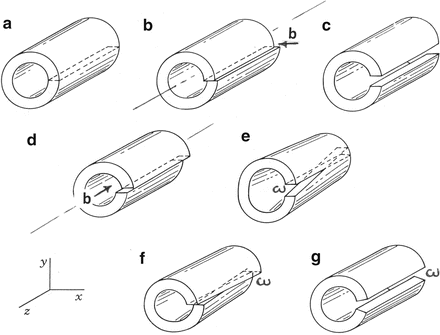
\includegraphics[width=0.5\textwidth]{imgs/fdm/voltera6.png}
        \caption{Line defects listed by Voltera \parencite{voltera1907}:  \emph{(a)} perfect cylinder, \emph{(b, c, d)} are translational defects (dislocations) and \emph{(e, f, g)} are rotational defects (disclinations).}\label{fig:voltera6}
\end{figure}
Following the discovery of X-rays and X-ray diffraction, the crystalline structure of metals was established. After that, strong evidences for the presence of dislocations emerged from efforts to reconcile theoretical and experimental values of the shear stress required for plastic deformation of a single perfect crystal. This can be traced back to \emph{Frenkel}'s work in 1926 \parencite{frenkelZurTheorie1926}. In an ideal crystal, the slip of one atomic plane over an adjacent plane would require a coordinated, rigid motion of all atoms from one position of perfect alignment to another. \emph{Frenkel} \parencite{frenkelZurTheorie1926} proposed that the shear force needed to slide the upper row of atoms over the lower row follows a periodic, sinusoidal function.
\begin{equation}
    \tau = \frac{G b}{2\pi a} \sin \frac{2\pi x}{b} \quad \Rightarrow \quad \tau_{max} = \frac{b}{a} \frac{G}{2\pi}
\end{equation}
This assumption revealed that the theoretical estimate of shear stress limit of a perfect crystal is several order of magnitude of those experimentally observed. This significant discrepancy between theory and experiment was explained in 1934 by the simultaneous and independent works of Orowan \parencite{Orowan34}, Polanyi \parencite{Polanyi34}, and Taylor \parencite{taylorMechanismPlastic1934} through the consideration of dislocations motion and its role in the mechanism behind plastic deformation of crystals. This also gave birth to the well-known model of caterpillar or carpet as an illustration to plastic deformation induced by dislocations motion in crystals, see \cref{fig:caterpilarPlasticity}.
\begin{figure}[H]
    \centering
    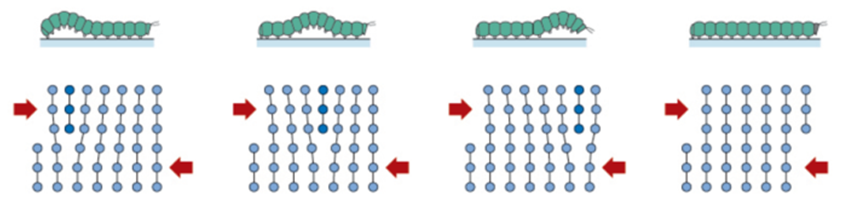
\includegraphics[width=0.9\textwidth]{imgs/fdm/caterpilar.png}
    \caption{Line defects listed by Voltera \parencite{voltera1907}:  \emph{(a)} perfect cylinder, \emph{(b, c, d)} are  dislocations and \emph{(e, f, g)} are disclinations.}\label{fig:caterpilarPlasticity}
\end{figure}
The existence of dislocations is also implied by studies of crystal growth. Studies of nucleation by Volmer (1939) followed the ideas of Gibbs (1948) and suggested that nucleation of new layers during growth of perfect crystals required supersaturations of about 1.5. However, experiments showed that crystals grew under nearly equilibrium conditions. The difficulty was resolved by Frank in 1949XX, by postulating that growth could proceed at lower supersaturations, by the propagation of ledges that are present where spiral dislocations intersect surfaces.\\
Since then, the presence and effects of dislocations have been recognized as significant. As a result, dislocations have been extensively studied to understand and quantify their impact on the properties of various material classes, including metals and semiconductors. Over the past fifty years, scientific advances have led to the development of methods for observing and modeling dislocations at different scales. Given the focus of this thesis on dislocation modeling, we will start by briefly reviewing the tools and models available in the literature for this purpose.
\subsection{Ab-initio modelling}
At the atomic level, quantum mechanics based models offer the most fundamental and accurate description of the underlying physics of dislocations. They're often deemed first principle calculations or Ab Initio simulations. These models rely on the so called \emph{Born-Oppenheimer} approximation: Atomic nuclei due to their mass, are assumed to be fixed and the problem is simplified into only solving for the evolution of the electrons by means \emph{Shrödinger}'s equation. \emph{Density Functional Theory} (DFT) is the most commonly used method for numerically solving \emph{Shrödinger}'s equation. Inferring to \emph{Hohenberg-Kohn} theorems \parencite{engelDensityFunctional2011} which allows one to bypass the need to solve for each electron individually, in DFT electrons' spatial distribution is replaced by as scalar function called electronic density which obeys Kohn-Sham equations.\\
There are available libraries such as, \emph{QuantumEspresso} or \emph{VASP} which allows optimized numerical solution to \emph{Kohn-Sham} equations. But DFT simulations remain computationally intensive, and scale cubically with the number of atoms, so that their often limited to few hundred of atoms. As a consequence, DFT calculations generally focus on dislocation core's structure \parencite{woodwardPredictionDislocation2008} and energy and give insight onto fundamental and local properties of dislocations such as cross slip, nucleation, selection of glide planes and mobility of dislocations \parencite{rodneyinitiomodeling2017}. Recently, these models explored quantum effects of atomic nuclei on lattice resistance in BCC materials \parencite{provilleQuantumeffect2012}, allowing better estimates and better understanding of \emph{Peierls stress} needed to move a dislocation within a plane of atoms. \\


In addition, these ab initio models have been widely used to generate material property databases for developing interatomic potentials \parencite{payneinitiodatabases1996}: a key ingredient for classical molecular dynamics models that operate at the next scale as presented in the following section.
\subsection{Molecular dynamics simulations}
At a molecular level, i.e on the scale of few hundreds of $nm$, \emph{molecular dynamics} (MD) and \emph{molecular statics} (MS) are used. Considered systems consists of classically described atoms interacting with each other with a given interaction potential $U$. The main variables are just atomic positions $\{\vecc{r_i}\}$ and their time evolution is prescribed by Newton's equation of motion:
\begin{equation}
    m_i \frac{d^2\vecc{r_i}}{dt^2} = - \vecc{\nabla}U(\vecc{r}) \quad \forall \, i
\end{equation}

Molecular dynamics have been widely used to study dislocations properties such as line energies \parencite{zhouAtomisticcalculations2017}, mobilities \parencite{olmstedAtomisticsimulations2004}, cross-slip rates \parencite{raoCalculationsintersection2011}, interactions between dislocations \parencite{zhouLargescalemolecular1998}, and with other defects \parencite{spearotInsightsslip2014}.\\
Optimized algorithm for the numerical integration of the equation of motion are commonly available today, such as \emph{LAMMPS} \parencite{thompsonLAMMPSflexible2022}. However, the major challenge in molecular simulations is post-processing: Analyzing atomic trajectories in order to identify dislocations from atomic positions. Algorithms, such as the \emph{Dislocation Extraction Algorithm} (DXA) \parencite{stukowskiExtractingdislocations2010}, automatically and efficiently detects dislocations and extracts their corresponding Burgers vector.\\


Although being less computationally expensive than ab initio methods, MD simulations of metals are still limited to systems of $\sim 10^6$ atoms. Moreover, integration of the equations of motion requires very small time steps ($\sim 1 \, fs$), so that the total duration of a simulation is around $10 ns$ if we perform $10^7$ timestep which limits the application of MD simulations to very high strain rate scenarios, usually $>10^6 \, s^{-1}$.
\subsection{Phase field crystal}
\subsection{Discrete dislocations dynamics}
At somewhat larger scale ($\sim \mu m$), a popular technique known as \emph{Discrete Dislocation dynamics} (DDD) \parencite{devincreThreeDimensionalSimulations1992} \parencite{kubinmodellingdislocation1992} is often used. It aims at retaining the discrete nature of dislocations in crystals while providing enough computational capabilities to exceed the time and space scale limitations of molecular simulations. The idea is to couple the motion of the discrete dislocations with a continuum elastic description of the medium in which they're embedded \parencite{bulatovComputerSimulations2006}.\\


Each dislocation line, let's say of index $i$, is discretized into $\lbrace\vecc{r_j}\rbrace_{1\leq j \leq N}$ node each with its own Burgers vector ${\vecc{b_{ij}}}$. At each time step, the stress field $\Tens{\sigma}$ is computed using linear elasticity which induces a Peach-Köehler force $\vecc{F_i}$ on each dislocation line to which some additional forces might be added if considered such as (Peierls, interaction, obstacle, osmotic, thermal, $\dots$). Using a mobility Law $\vecc{V_i}=M(\vecc{F_i^{tot}})$, the position of each dislocation is updated by a time integration of :
\begin{equation}
    \frac{d \vecc{r_i}}{dt} = g_i(\lbrace\vecc{r_j}\rbrace,\dots)
\end{equation}
After updating the position of each dislocation line, a special algorithm is needed to keep track of all dislocations and detects' possible collisions. Following this step, a set of well-defined and prescribed rules is used to handle interactions and topological changes such as junction formations, intersections, annihilation, cross slip, nucleation etc... Optimized open-source codes are available to perform DDD simulations like ParaDiS \parencite{paradis} developed at Stanford University, and TriDis \parencite{tridis} developed at SIMaP in Grenoble. Even though \emph{GPU} acceleration has been proposed \parencite{bertinGPUaccelerateddislocation2019} which allowed large scale DDD simulations within reasonable running time, computational cost is still too high if one aims at replicating the strain rates typically used in experimental setups. Recently, an attempt has been proposed by coupling DDD to Finite elements \parencite{cuiDislocationevolution2021}, in order to study Dislocation evolution during thermo-mechanical loading of tungsten.

\subsection{Continuous distribution of dislocations}
Before attempting to move to a larger scale, it is important to have an estimate of the amount of dislocations stored in crystal. For this aim, we introduce a scalar quantity : the dislocation density $\rho^d$ which is the defined as the total length of all dislocation lines per unit volume. In an undeformed metal, the dislocation density is often $\sim 10^8\, m^{-2}$, However heavily deformed metals exhibits high dislocation densities  $\sim 10^{15}\, m^{-2}$ \parencite{kochmannMechanicalmodeling2009}. Due to this high density, it would be inefficient and quite impossible to handle the excessive amount of dislocations when working in scale of $\sim cm$, for which the total length of dislocation lines would be around $1000\,km$. For this purpose, the static continuum theory of dislocations was introduced by \emph{Nye} \parencite{nyeGeometricalRelations1953}, \emph{Bilby} \parencite{bilbly1955}, \emph{Kröner}\parencite{kroenerAllgemeineKontinuumstheorie1959} and \emph{Willis} \parencite{willisSecondordereffects1967a}, and further formalized using modern statistical mechanics and thermodynamics by \emph{Berdichvsky} \parencite{berdichevskyContinuumtheory2006}.\\


The continuum theory  of dislocations treats the behavior of the large ensemble of dislocations in the medium by means of common continuum mechanics, using an explicit dependence of the free energy of the system on the dislocations density. The tenet of the theory is the so called dislocation density tensor $\Tens{\alpha}$ introduced by \emph{Nye} \parencite{nyeGeometricalRelations1953} to take into account the \emph{geometrically necessarily dislocations} (GNDs). Nye used geometrical arguments to link the curvature tensor $\Tens{\kappa}$ to the dislocation density tensor $\Tens{\alpha}$:
\begin{equation}
    \Tens{\kappa} = \Tens{\alpha}- \frac{1}{2} \Tr \Tens{\alpha} \, \Tens{\mathbb{I}}
\end{equation}
Kröner \parencite{kroenerAllgemeineKontinuumstheorie1959} formalized the definition of the dislocation density tensor $\Tens{\alpha}$ as the fundamental measure of incompatibility, and established its link with and the plastic distortion $\Tens{U^p}$ in a small deformation setting.\\
Given a surface $\mathcal{S}$ inside the medium bounded by a closed circuit $\mathcal{C}$, he noted that :
\begin{equation}
    \iint_\mathcal{S} \Tens{\alpha} \cdot \vecc{da}=\iint_\mathcal{S} \Trot \Tens{U^p} \cdot \vecc{da} = \oint_\mathcal{C} \Tens{U^p} \cdot \vecc{dl} = \vecc{b_c} \quad \text{with} \quad \Tens{\alpha} := \Trot \Tens{U^p}
\end{equation}
Following this definition, the dislocation density tensor $\Tens{\alpha}$ is a second order tensor that gives for any arbitrary closed circuit $\mathcal{C}$ the resulting Burgers vector $\vecc{b_c}$ of all dislocation lines threading through it. Which suggests to interpret $\Tens{\alpha}$ as line density where each line carries some Burgers vector, so that locally, at least, we can write $\Tens{\alpha}=\vecc{b_c} \otimes \vecc{t}$ where $\vecc{t}$ is the tangent vector to a dislocation line, or the normal vector to an infinitesimal surface $\vecc{da}$. \\
After introducing $\Tens{\alpha}$, the first problem addressed was on how to find the stress field produced by a given dislocation density $\Tens{\alpha}$. It was elegantly solved by \emph{Kröner} \parencite{kroenerAllgemeineKontinuumstheorie1959} in 1598 in a linear setting. Then, the same problem was solved by Willis \parencite{willisSecondordereffects1967} but in a finite deformation framework while also accounting for material anisotropy.\\


The so far presented works only apply for the static case. It was only due to the work of \emph{Mura} \parencite{muraContinuousdistribution1963} in 1963, \emph{Fox} \parencite{foxContinuumTheory1966} in 1966 and \emph{Kosevich} \parencite{kosevichDYNAMICALTHEORY} in 1979, that a full dynamical theory of moving dislocations was established. The authors, from different derivations, obtained the following evolution equation of the dislocation density tensor:
\begin{equation}
    \dot{\Tens{\alpha}}= - \Trot \left( \Tens{\alpha}\times \vecc{v^d}\right)
\end{equation}
Where $\vecc{v^d}$ is the dislocation velocity vector. The term $\Tens{\alpha}\times \vecc{v^d}$ was interpreted as \emph{dislocation flux density} by \emph{Kosevich} \parencite{kosevichDYNAMICALTHEORY}, and was understood as the plastic strain rate induced by dislocation motion. The physical interpretation was further analyzed by \emph{Acharya} in \parencite{acharyaMicrocanonicalEntropy2011}.\\


It was quickly understood that the continuum theory of dislocations raises a fundamental issue when treating the dislocation core : Stresses diverges within the core, the incompatible elastic displacement is discontinuous and more importantly the core cannot be kept compact and localized. The issue was first addressed by \emph{Peierls} in 1940 \parencite{peierlssizedislocation1940}, in the case of a single edge dislocation. If the core is represented as a continuous distribution, the stress around it tend to spread it out independent and equilibrium structure of the core can be maintained. This can be understood using the fact that two dislocations of the same sign tend to repel each other so that a continuous description of the core of a single dislocation will naturally diffuse until it uniformly vanishes. Peierls \parencite{peierlssizedislocation1940} argued that a stable compact core is maintained if the internal stress from the continuous distribution is balanced by a restoring force that reflects the underlying crystal structure. His model was later extended by \emph{Nabarro} \parencite{nabarroDislocationssimple1947} in 1947, which became the well known \emph{Peierls-Nabarro} model. The model introduced a sinusoidal restoring stress $T^R$ that depends on the misfit $\eta$, originally introduced for an edge dislocation in a infinite simple cubic crystal :
\begin{equation}
    T^R = \frac{\mu}{2 \pi} \sin \left(2 \pi \frac{\eta}{b} \right) \quad  \text{with} \quad \eta(x) = \frac{b}{2}+\frac{b}{\pi} \arctan \left( 2(1-\nu \frac{x}{b})\right)
\end{equation}
In addition, this resorting stress can be used to construct a regularization of total elastic energy in order to treat the discontinuity of the incompatible elastic displacement within the core of the dislocation. The new term adds a non-convex part to the total energy \parencite{fressengeasMechanicsdislocation2017}, from which an equilibrium compact core can be found. It reads:
\begin{equation}
    \Psi = \psi(\epsilon^e) + \frac{\gamma}{d} \quad \text{with} \quad \gamma = \frac{\mu b }{4 \pi^2} \left( 1- \cos \left(2 \pi \frac{\eta}{b} \right) \right)
\end{equation}
Furthermore, one of the major shortcomings of the theory of continuously distributed dislocations is the resolution size dependence on the Burgers circuit $\mathcal{C}$ used to detect dislocations, the main issue being that only the resulting Burgers vector is measured through $\Tens \alpha$ \parencite{kronerBenefitsshortcomings2001}. This means that all the positive and negative dislocations cancel each other to a very large amount. The Kroner-Nye dislocation tensor only captures, if one works on a meso/macroscale, the so called geometrically necessary dislocations (GNDs) and overlooks all the statistically stored dislocations (SSDs) \parencite{sandfeldContinuummodeling2011}. As a result, it overlooks the complex internal structure of the dislocation network, leading to an incomplete description of the internal mechanical state. As a consequences, all theories based on the \emph{Kröner-Nye} tensor need to be patched up by phenomenological terms to take into account averaged out dislocations when modeling meso/macroscale plastic deformations. An example is the phenomenological mesoscale field dislocation mechanics suggested by \emph{Acharya} and \emph{Roy} \parencite{acharyaSizeeffects2006}. The dislocation transport of the mesoscopic space-times averaged field variables $\Tens{\overline{\alpha}}$ and $\overline{\vecc{V}}^d$ is given by \parencite{acharyaSizeeffects2006}:
\begin{equation}
    \mathring{\Tens{\overline{\alpha}}} = - \Trot \left( \Tens{\overline{\alpha}} \times \overline{\vecc{V}}^d+ \Tens{L^p}\right)+\Tens{s}
\end{equation}
Where $\Tens{L^p}$ is the plastic strain rate produced by the statistical dislocations (microscopic) which is not accounted for in $\Tens{\overline{\alpha}} \times \overline{\vecc{V}}^d$, and $\Tens{s}$ is a dislocation nucleation rate term. Both $\Tens{L^p}$ and $\Tens{s}$, (as well as dislocation velocity) should be prescribed constitutively depending on the desired model. Examples of $J2$ plasticity and crystal plasticity are given in \parencite{aroraComputationalApproximation2019}.

\subsection{Continuum dislocation dynamics}
It was already pointed out that the classical \emph{Kröner-Nye} dislocation tensor averages overall several dislocation lines to yield their resultant Burgers vector \parencite{kronerBenefitsshortcomings2001} , so that information on the microscopic statistical dislocations is lost. In addition, it is important to understand that the kinematic information stored in $\Tens \alpha$ is only reliable if all dislocation lines threading through the circuit are parallel: if they differ in orientation the resulting average is necessarily altered.\\


A different apporoach proposed by \emph{Hochrainer} \parencite{hochrainerthreedimensionalcontinuum2007} \parencite{hochrainerContinuumdislocation2014}, in his continuum dislocation dynamics theory. He introduces what he calls the \emph{second order dislocation density tensor} (\textbf{SODT}) $\Tens{\alpha}^{II}$ that lives on higher dimensional space ($\mathbb{R} \otimes \mathbb{R} \otimes \mathbb{S}^1$), in contrast to $\Tens{\alpha} \in \mathbb{R} \otimes \mathbb{R}$. The SODT $\Tens{\alpha}^{II}$  distinguishes dislocations a priori by their line direction before any averaging is introduced: it consider the angle $\varphi$ between the tangential vector $\vecc{t}$ and its Burgers' vector $\vecc{b}$. Hence, it is able to describe the kinematics of very general systems of dislocations. It was shown that the SODT simplifies to the classical \emph{Kröner-Nye} tensor. The former is uniquely defines by the scalar dislocation density $\rho^d$ and the curvature density $\kappa^d$, which are also used to derive coupled evolution equations.

\subsection{Field dislocation mechanics}
\emph{Field dislocation mechanics} (\textbf{FDM}) is a continuum theory for crystal plasticity proposed by \emph{Acharya} in 2001 \parencite{acharyamodelcrystal2001} following the works of \emph{Willis} \parencite{willisSecondordereffects1967}, \emph{Kröner} \parencite{kroenerAllgemeineKontinuumstheorie1959}, \emph{Fox} \parencite{foxContinuumTheory1966}, \emph{Mura} \parencite{muraContinuousdistribution1963} and \emph{Kosevich} \parencite{kosevichDYNAMICALTHEORY}. As explained in \parencite{acharyamodelcrystal2001}, FDM is introduced as an attempt to extend and improve the \emph{elastic theory of the continuously distributed dislocations} (\textbf{ECDD}) presented in \parencite{willisSecondordereffects1967} for which the main issue is the lack of the two-way interaction between stress state and dislocation field. In addition, the problem as initially posed in ECDD is ill-posed : given an inverse elastic distortion $\Tens W$, one can compute a unique dislocation field $\Tens \alpha$; however, given $\Tens \alpha$, uniqueness of $\Tens W$  is lost because they're related by $ \Trot \Tens{W} = - \Tens{\alpha}$ and $\Tens W + \Tens \nabla \vecc{f}$ is a solution for any vector field $\vecc{f}$. The idea behind \emph{Acharya}'s work in an orthogonal decomposition using the null space of the $\Trot$ operator of tensors into compatible and incompatible parts, which enables a unique determination of the deformation field by adding an additional equation governing $\Tens \nabla \vecc{f}$ using constitutive analysis as performed by \emph{Acharya} in \parencite{acharyaConstitutiveanalysis2004}. The inverse elastic distortion is decomposed into compatible and incompatible parts (which will later on understood as a generalization of Stokes-Helmholtz decomposition to higher order tensors):
\begin{equation}
\begin{aligned}
&\Tens W= \Tens\chi + \Tens \nabla \, \vecc f  \quad \text{with} \quad \Tens W = \Tens{F_e}^{-1}\\
& \Trot \Tens W= \Trot \Tens \chi = -\Tens \alpha \\
&\Tdiv \Tens \chi = 0 \\
&\Tdiv (\Tens \nabla \dot{\vecc{f}})= \Tdiv   (\Tens \alpha \times \vecc{v^d} - \dot{\Tens \chi} -\Tens \chi  \Tens L)
\end{aligned}
\end{equation}
The constitutive analysis also exposes the driving force acting on the dislocations as a non linear generalization of the classical \emph{Peach-Koehler} forces \parencite{acharyaDrivingforces2003}, \parencite{acharyaConstitutiveanalysis2004}:
\begin{equation}
        \vecc{f^d} := \rho \left(\frac{\partial \psi}{\partial \Tens W}\right) ^t\Tens{\alpha} : \Levi{}
\end{equation} 
In addition, the dislocation transport equation used is the same as the one derived by \emph{Mura} \parencite{muraContinuousdistribution1963} and \parencite{kosevichDYNAMICALTHEORY}, i.e 
$\dot{\Tens{\alpha}}= - \Trot \left( \Tens{\alpha}\times \vecc{v^d}\right)$. In \parencite{acharyaDrivingforces2003}, \emph{Acharya} derives the necessary boundary conditions on $\Tens \alpha$ for the closure of the dislocation transport equation which reduces to the specification of the dislocation flux $\vecc{v^d}\cdot \vecc{n}\Tens \alpha = F_\alpha $ on the inflow boundary $\partial \Omega_t^-$ where $\vecc{v^d}\cdot \vecc{n} <0$. In its early stages and shortly after its foundation had been posed,  FDM theory proved itself by successfully representing various physical features such as local Schmid and non-Schmid behaviors, yielding \parencite{acharyaDrivingforces2003}, and the formation of a slip step when a moving dislocation meets a free surface boundary \parencite{acharyamodelcrystal2001}. In addition, it was shown that the theory reduces to classical non linear elasticity when no dislocations are involved, and to classical theory of continuously distributed dislocations when no velocity is considered \parencite{acharyaConstitutiveanalysis2004}. One of the main advantages of FDM, is that dislocations are treated as a continuous field and their time evolution is PDE-dictated, bypassing any need to prescribe interaction rules (like those used in DDD) So that the increasing number of dislocations has no computational cost. As demonstrated in \parencite{varadhanDislocationtransport2006}, the transport equation used in FDM is able to model expansion, annihilation and shocks of dislocations. Another conceptual advantage, is that FDM do not introducing neither an intermediate nor a reference configuration, so that the multiplicative decomposition of the distortion into plastic $\Tens{F}_p$ and elastic $\Tens{F}_e$ is not postulated \parencite{acharyadislocationmotion2015}. Instead, it is assumed that at each time step, the body can be, by thought, mapped to a relaxed stress free configuration which is fictitious and not necessarily connected. The relaxed configuration serves as a way to introduce the (inverse) elastic distortion and the Burgers vector \parencite{fressengeasMechanicsdislocation2017}: A closed curve in the current configuration is not necessarily closed when pulled-back to the relaxed one, the failure in closure is the Burgers vector given in units of the undeformed lattice in the relaxed configuration. Even though no multiplicative decomposition is postulated in the theory, an additive decomposition of the velocity gradient naturally emerges from the conservation of Burgers vector  \parencite{acharyadislocationmotion2015}.\\


Field dislocation mechanics is continuum theory in which kinetic energy of atomic vibrations (and all energy below a given length scale) have been averaged out exchanged with a dissipative evolution of continous density fields encoded in the mathematical structure of the PDEs governing the evolution \parencite{acharyaNewinroads2010}. The theory was introduced as an attempt to model crystal plasticity at a time scale of $\sim \mu s$ and more, however it was previously argued the averaged nature of the theory makes it unvalid at larger length scales since it doesn't account for the statistically stored disclocations and it is necessary to back it up with phenomenological assumptions. It is in this puropose that the phenomenological mesoscopic field dislocation mechanics was introduced in 2006 \parencite{acharyaSizeeffects2006}. The newly introduced theory is merely a space-time average of the previously developed Field dislocation mechanics followed by closure assumptions, and by constitutive prescription of the plastic strain rate of the statistically stored dislocations. With that being said, FDM can be seen a bridge between elastolpasticity and dislocation theory which were always treated as separate topics, it also includes several physical aspecets of crystal plasticty. Nonetheless, There are still some fundamental issues to be adressed, namely on relevance of the core energy regulariziation \parencite{acharyaequationtheory}, on the existence of a \emph{Peierls} stress threshold to the onset of  dislocation motion which was proved to exist in some special cases \parencite{acharyaNewinroads2010} \parencite{zhangsingletheory2015}, on the inclusion of crystalline structure in order to keep a compact core \parencite{acharyaNewinroads2010}, and the speed of propagation of elasatic waves in the dynamis of dislocations \parencite{zhangsingletheory2015}. Additionally, the FDM theory as porposed and developed through the years remained isothermal until the \emph{Thermal-FDM} was porposed by \emph{Upadhyay} in \parencite{upadhyaythermomechanicaltheory2020}. \emph{Thermal-FDM} (\emph{T-FDM}) introduces a strong coupling between dislocation mechanics and heat conduction, targeting dislocation dynamics under rapid or gradual temperature changes, such as in heat-affected crystalline solids during additive manufacturing, to model temperature changes can drive dislocation behaviors, and vice versa.\\

The first numerical implementation of field dislocation mechanics (FDM) goes back to \emph{Roy} and \emph{Acharya} in 2005 \parencite{royFiniteelement2005}, who developed a finite element solver for both static and moving dislocations within the small deformation limit, albeit with a constant velocity constraint (since stress coupling hindered maintaining a compact dislocation core). Then, the following studies focused on the dynamics of dislocation transport, such as the work by \emph{Varadhan} \parencite{varadhanDislocationtransport2006}, which explored a purely kinematic dislocation evolution, where velocity and stress fields were also uncoupled. Their simulations demonstrated that FDM accurately captured essential behaviors like shock formation, wave propagation, and annihilation events, as seen in the expansion of a polygonal loop and the operation of a \emph{Frank-Read} source. It was until 2020, that \emph{Arora} developed a finite element implementation of the mesoscopic field dislocation mechanics capable of handling large deformations \parencite{aroraFiniteelement2020}. Their work first demonstrated non-linear elasticity in dislocation-free conditions, then it was used to analyze stress fields in cases involving isolated dislocations and homogenous dislocation densities. They numerically confirmed that a spatially homogenous dislocation density is not stress-free when geometric non-linearities are taken into account, corroborating previous theoretical predictions \parencite{acharyaStressspatially2018}. Furthermore, the model successfully reproduced the formation of slip steps and shear bands without ad-hoc failure criteria in the stress-uncoupled case, along with Mach cone formation for supersonic dislocation velocities. This implementation of mesoscopic FDM also demonstrated the emergence of complex dislocation patterns and realistic microstructural features of crystal plasticity \parencite{aroraDislocationpattern2020}. To tackle the stress-coupled case, \emph{Arora} introduced a non-convex term (see \cref{eq:regaurora}) inspired by the \emph{Peierls-Nabarro} model \parencite{nabarroDislocationssimple1947}, which depends a new state variable $\Tens P$, enabling the annihilation of two edge dislocations while maintaining a compact core \parencite{aroraComputationalApproximation2019}. 
\begin{equation}\label{eq:regaurora}
    \psi(\Tens W, \Tens \alpha, \Tens P) = \varphi_e(\Tens W) + \Upsilon(\Tens \alpha) +  \underbrace{\eta(\Tens  P)}_{\text{extra term}} \quad \text{with} \quad \eta(\Tens  P) = \frac{C}{\rho^*} \left[ 1- \cos \frac{2 \pi P_{12}}{\omega}\right]
\end{equation}

Most recently, a finite element implementation of the small deformation limit of thermal field dislocation mechanics (T-FDM) was achieved, expanding on previous isothermal models by integrating temperature effects. The model allows for explicit simulation of how dislocations impact temperature profiles and vice versa \parencite{lima-chavesFiniteelement2024}.\\

Despite its promising framework for simulating dislocation mechanics without ad-hoc interaction rules, \emph{Field Dislocation Mechanics} (\textbf{FDM}), has some essential limitations. Previously, we identified a major limitation: FDM does not inherently account for the underlying crystalline structure of the material. This limitation affects the ability of dislocation cores to remain compact and hinders the coupling between stress and dislocation velocity. To address this, a coupling between FDM and the \emph{Phase Field Crystal} (\textbf{PFC}) model was proposed \parencite{acharyaFielddislocation2020}. The PFC model, a phase-field approach within the domain of complex pattern formation, employs a \emph{Swift-Hohenberg} type of energy functional, which is minimized to generate a desired crystalline structures. Integrating PFC with FDM introduces a non-convex energy term that enhances the representation of crystal structures within the formulation of FDM. Prior to diving into the specifics of the PFC-FDM coupling, we first provide in the upcoming section an overview of pattern formation theories and the PFC model.
\subsection{Field dislocation mechanics and phase field crystal}

\section{Modelling tools summary}
\begin{center}
    \renewcommand{\arraystretch}{1.4}
\begin{table}[H]
\begin{tabular}{|c|c|c|c|c|c|}
\hline
\textbf{Technique}                     & \textbf{Length scale}            & \textbf{Time scale}                                       & \textbf{Crystal.}                             & \textbf{Evolution}                                        & \textbf{Elasticity}                                  \\ \hline
\textit{Q-DFT}                     & \cellcolor{Nocell}$\mathring{A}$   & \cellcolor{Nocell}$fs$                                 & \cellcolor{Yescell}Natural                          & \cellcolor{Yescell}{Kohn-Sham} & \cellcolor{Yescell}{ Yes} \\ \hline
\textit{MD}            & \cellcolor{Yescell}$nm$       & \cellcolor{Nocell}$\sim ps, \sim ns$                              & \cellcolor{Yescell}Natural                          & \cellcolor{Yescell}{Newton} & \cellcolor{Yescell}Yes                          \\ \hline
\textit{PFC}                           & \cellcolor{Yescell}$nm$       & \cellcolor{Yescell}Diffusive                          & \cellcolor{Yescell}Natural                          & \cellcolor{Yescell}{Disspative Flow}        & \cellcolor{Nocell}No                           \\ \hline
\textit{DDD} & \cellcolor{Yescell}$\mu m$       & \cellcolor{Yescell}$ns $                                 & \cellcolor{Nocell}Prescribed                           & \cellcolor{Nocell}Kinetic laws                        & \cellcolor{Yescell}Yes                          \\ \hline
\textit{FDM}                           & \cellcolor{Yescell}Mesoscale & \cellcolor{Yescell}Diffusive/Quasi-static                & \cellcolor{Nocell}Prescribed                           & \cellcolor{Yescell}Conservation laws                               & \cellcolor{Yescell}Yes                         \\ \hline
\textit{CP}            & \cellcolor{Nocell}$\sim \mu m, \sim mm$    & \cellcolor{Yescell}{ Quasi-static } & \cellcolor{Nocell}{Prescribed} & \cellcolor{Nocell}Constitutive+Rules               & \cellcolor{Yescell}Yes                          \\ \hline
\end{tabular}
\end{table}
\end{center}
\end{document}